\chapter{Oracle实践}

\section{Oracle介绍}
版本介绍:\\
Oracle 8i表示向网络方向发展
Oracle 9i是Oracle 8i的稳定版,3CD。
Oracle 10g表示向网格计算(更高效的搜索算法)发展。
Oracle 11g是10g的稳定版,是最主流的广泛。
Oracle 12C,最新的版本是,表示云计算(cloud),本次将课使用11g版本。

\section{Oracle安装}
准备出5G的空间。

防止日后的程序乱码,字符集选择UTF-8
\begin{figure}[H]
  \centering
  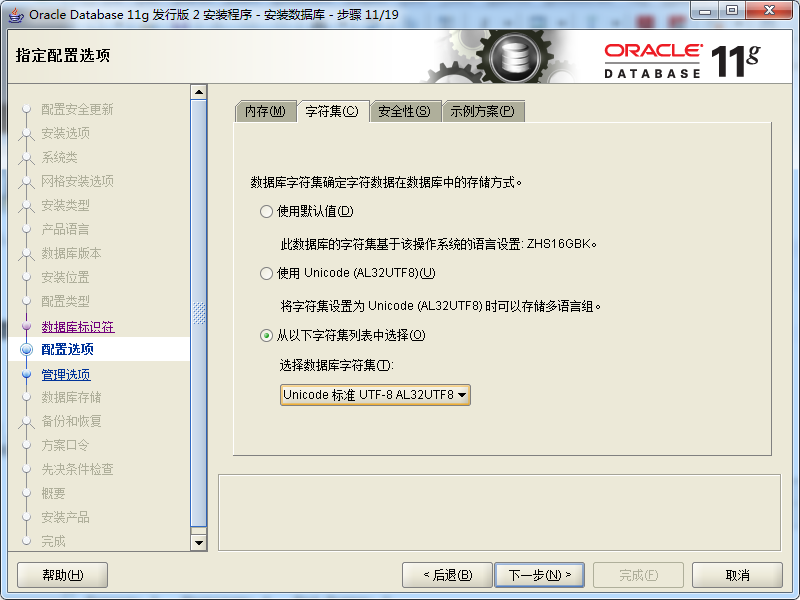
\includegraphics[width=10cm]{oracle/安装步骤_指定配置_选择字符集.png}
%  \caption{}\label{}
\end{figure}
接下来事例方案选项卡中选择创建具有事例方案的数据库。比较重要。
\begin{figure}[H]
  \centering
  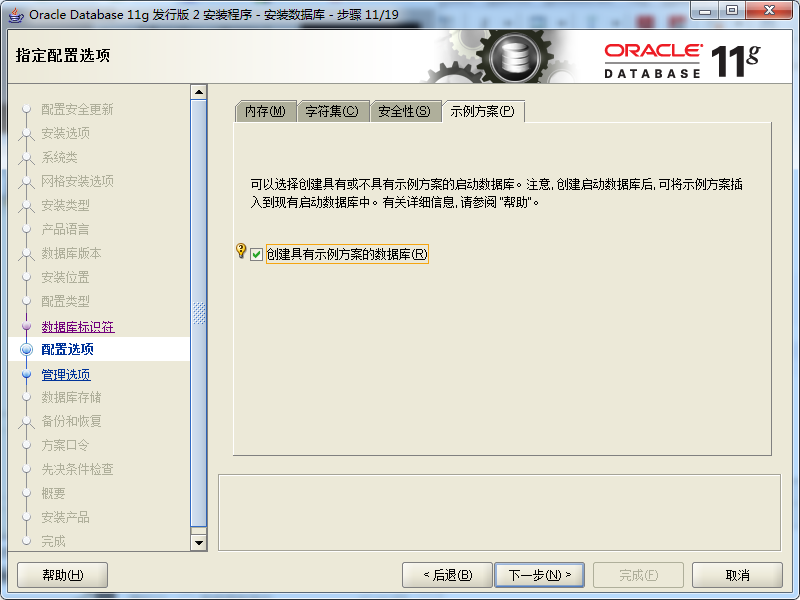
\includegraphics[width=10cm]{oracle/安装步骤_指定配置_选择创建示例方案.png}
%  \caption{}\label{}
\end{figure}

接下来是配置口令,不同的管理员可以设置不同的密码,但是现在我们设置一样的密码,我的密码是241833Ab。

四个主要的用户
\begin{itemize}
  \item sys 超级管理员
  \item system 普通管理员
  \item scott 普通用户
  \item sh 大数据用户
\end{itemize}

\begin{figure}[H]
  \centering
  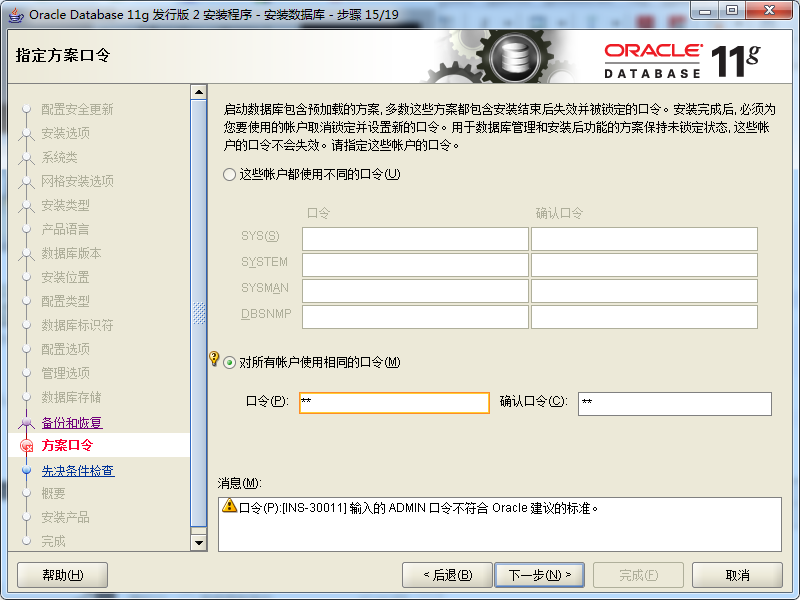
\includegraphics[width=10cm]{oracle/安装步骤_指定配置_配置口令.png}
%  \caption{}\label{}
\end{figure}

然后就是环境检测,即使环境检测结果有问题也没有关系,可以跳过,进行安装。安装的时候可能会弹出一些错误点击忽略。记得拖滚动条选择SCOTT账号,设置密码。
安装完成后进行口令管理:
\begin{figure}[H]
  \centering
  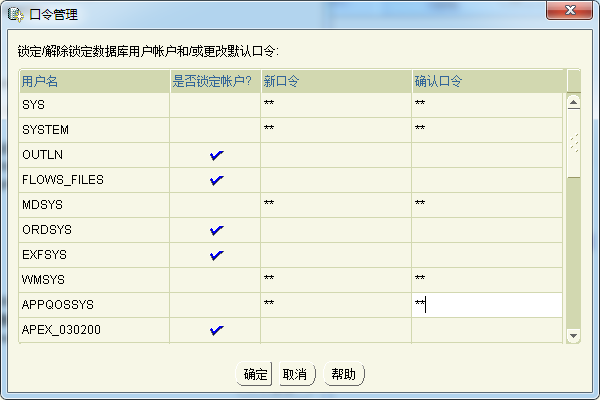
\includegraphics[width=10cm]{oracle/口令管理.png}
%  \caption{}\label{}
\end{figure}
最后点击安装完成。


\section{Oracle操作}

\subsection{进入控制台}
打开控制台,输入sqlplus.exe,然后输入账号scott和密码fe:
\begin{figure}[H]
  \centering
  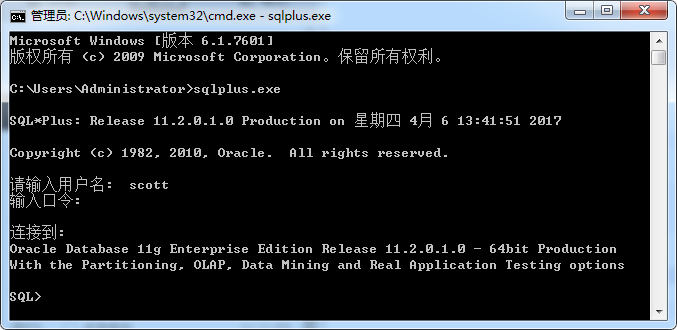
\includegraphics[width=10cm]{oracle/打开sqlplus.png}
%  \caption{}\label{}
\end{figure}

\subsection{SQLPLUS基本命令}
格式调整命令,解决显示混乱的问题:
\begin{verbatim}
SQL> select * from emp;     #不区分大小写,此时显示不清楚,有断行
SQL> set linesize 300;      #设置每行的宽度
SQL> set pagesize 30;       #设置每页的行数
\end{verbatim}

调用记事本命令(将命令打包):
\begin{verbatim}
SQL> ed 文件名称                                    #创建一个记事本,将命令放在里面,批量执行
SQL> @文件名.sql             #执行该文件
SQL> @d:\文件名.sql          #执行磁盘上的某个数据库脚本文件
\end{verbatim}

用户管理命令:
\begin{verbatim}
SQL> show user              #显示当前用户
SQL> conn sys/fe as sysdba  #切换到sys这个用户,fe是密码
SQL> conn scott/fe          #切换回scott
\end{verbatim}

调用本地机器命令,但是要在之前加上host.
\begin{verbatim}
SQL> host mkdir test
\end{verbatim}
\subsubsection{引用的例子}
这是一个引用~\cite{LCN2002}

scott用户的主要数据表(***)。  一个数据库中有大量的表。
\begin{verbatim}
SQL> select * from tab;     #查询某个用户下的所有表
SQL> desc dept              #查看表的结构
SQL> select * from dept;    #查看表的内容
SQL> select * from emp;
SQL> select * from salgrade;
\end{verbatim}
\begin{figure}[H]
  \centering
  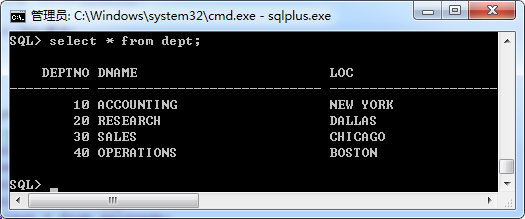
\includegraphics[width=8cm]{oracle/table_dept.png}
%  \caption{}\label{}
\end{figure}
\begin{figure}[H]
  \centering
  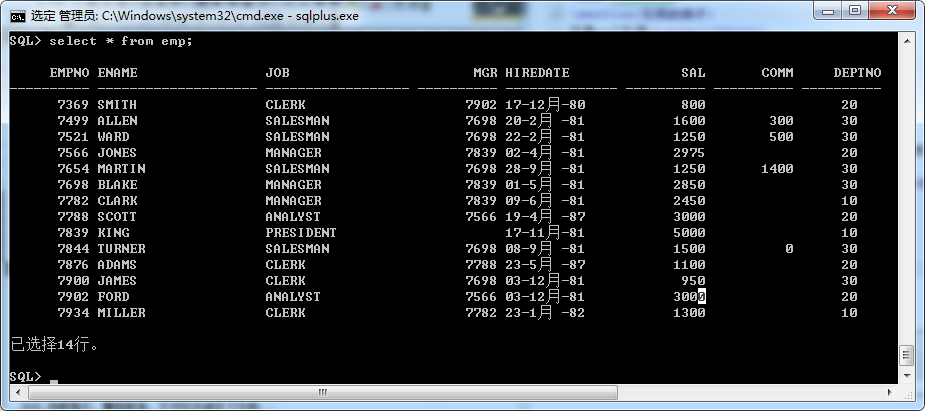
\includegraphics[width=14cm]{oracle/table_emp.png}
%  \caption{}\label{}
\end{figure}
\begin{figure}[H]
  \centering
  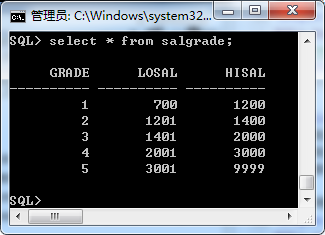
\includegraphics[width=8cm]{oracle/table_salgrade.png}
%  \caption{}\label{}
\end{figure}

\section{SQL几种查询操作}

\subsection{简单查询}
\begin{verbatim}
SELECT[DISTINCT] * || 列 [别名],列 [别名],...
FROM 表名称 [别名]

SQL> select * from emp;     #其实这是2个语句,from是子句
SQL> select empno,ename,job,sal from emp;
                            #查询特定的几个列,回避中文
SQL> select  empno,ename,sal*12 年薪 from emp;
                            #其中可以进行计算,空格之后可以加别名
简单查询,显示全部的数据行。

使用distinct去掉重复列(在所有的列都重复的情况下才会消除)\\
SQL> select distinct job from emp;

连接符:||,表示把数据连接合并起来
select '编号:'||empno from emp;
\end{verbatim}

\subsection{限定查询}
限定查询,所谓的限定查询就是添加一个查询的条件而已。
\begin{verbatim}
SELECT[DISTINCT] * || 列 [别名],列 [别名],...
FROM 表名称 [别名]
[WHERE 条件(s)]
\end{verbatim}

\subsection{基数查询}
\begin{verbatim}
SELECT * FROM emp
WHERE empno IN(7369,7566);

SELECT * FROM emp                       #切记,NOT IN中不能有NULL
WHERE empno NOT IN(7369,7566,NULL);     #原因是数据库自身的保护机制,避免大数据带来的问题。
\end{verbatim}

\subsection{模糊查询}
模糊查询 LIKE,正则表达式来查询
\begin{verbatim}
'_':匹配任意一个字符。
'%':匹配0个,1个或者多个任意字符。

SELECT * FROM emp
WHERE ename LIKE 'A%';
\end{verbatim}

\subsection{查询排序}
\begin{verbatim}
SELECT * FROM emp
WHERE ename LIKE 'A%';
ORDER BY 字段 [ASC|DESC],...
\end{verbatim}

\subsection{交互式查询}
\begin{verbatim}
交互式查询,用户指定查询的数据的名称。(**)
SELECT * FROM &tablename;
要注意大小写,和双引号。

SELECT * FROM emp
WHRER ename=&name;          #这样子是查不出来的,因为名字是要有双引号

SELECT * FROM emp
WHRER ename='&name';        #要输入名字,且要注意大小写

SELECT * FROM emp
WHRER ename=UPPER('&name'); #这样是完美的的,将字符转换为大写
SELECT * FROM emp
WHRER ename=LOWER('&name'); #这样是完美的的,将字符转换为小写
SELECT * FROM emp
WHRER ename=INICAP('&name'); #首字母大写,其他的小写
\end{verbatim}

DML(**),又称为DQL
DDL(**)
DCL,一般由DBA负责。